\documentclass{standalone}
\usepackage{tikz}
\usetikzlibrary{shapes.geometric,arrows.meta,bending,positioning}
\tikzset{
  >=latex,
  line/.style={->},
  line/.default=black,
}

\begin{document}
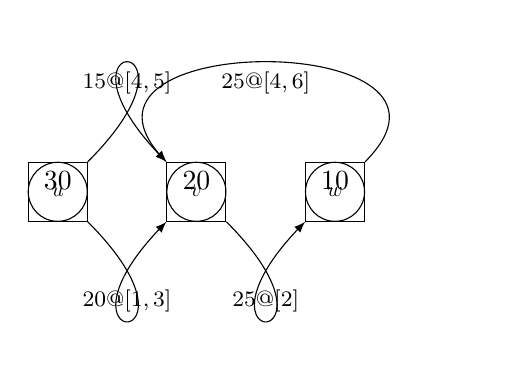
\begin{tikzpicture}[scale=0.8]
    % Node definitions
    \node[
        draw,
        minimum size=1cm,
        circle,
        scale=0.75
    ] (u) {$u$};
    \node[
        draw,
        minimum size=1cm,
        inner sep=1pt,
        rectangle,
        label={[anchor=north]north:$30$},
        scale=0.75
    ] at (u) (u-box){};
    \node[
        draw,
        minimum size=1cm,
        circle,
        right=of u,
        scale=0.75
    ] (v) {$v$};
    \node[
        draw,
        minimum size=1cm,
        inner sep=1pt,
        rectangle,
        label={[anchor=north]north:$20$},
        scale=0.75
    ] at (v) (v-box){};
    \node[
        draw,
        minimum size=1cm,
        circle,
        right=of v,
        scale=0.75
    ] (w) {$w$};
    \node[
        draw,
        minimum size=1cm,
        inner sep=1pt,
        rectangle,
        label={[anchor=north]north:$10$},
        scale=0.75
    ] at (w) (w-box){};
    % Edge definitions
    \draw[line] (u-box) to [out=-45,in=-135,distance=3cm] node[above]{\footnotesize{$20@[1,3]$}} (v-box);
    \draw[line] (v-box) to [out=-45,in=-135,distance=3cm] node[above]{\footnotesize{$25@[2]$}} (w-box);
    \draw[line] (w-box) to [out=45,in=135,distance=3cm] node[below]{\footnotesize{$25@[4,6]$}} (v-box);
    \draw[line] (u-box) to [out=45,in=135,distance=3cm] node[below]{\footnotesize{$15@[4,5]$}} (v-box);
\end{tikzpicture}
\end{document}